\chapter{Literature Review} 
% Main chapter title

\label{Chapter2} 
%Call reference to this chapter use \ref{ChapterX}

\lhead{Chapter 2. \emph{Literature Review}} 
% Change X to a consecutive number; this is for the header on each page - perhaps a shortened title

\doublespacing
% LINE FORMATTING


\section{Sequencial Programming vs Concurrent Programming}

Sequential programming involves process execution one after another \cite{control-structures} and have no linguistic design construct for concurrent computations. \cite{sequential-vs-concurrent} The processes will only run after other is successful and executed chronologically in predetermined manner. \cite{sequential-programming} However, it’s difficult to implement complex interaction and handle problems in parallel and concurrent environments with single-threaded. \cite{concurrency-revolution-in-sd} 

Concurrency had cause major turning point force in software development for developing concurrent software in order to exploit greater efficiency and performance optimization by fully utilize multiple core. To leverage the full power of hardware resource in software industry, concurrency and clouds will be the things every developer requires to deal with future software development and it is essential for both concurrent and distributed system.  \cite{concurrent-distributed-programming-in-future} Future generation computing system likely being developed by concurrent programming on multiprocessors. \cite{oop-concurrent} 

\section{Concurrent Programming}

Concurrent programming is form of computing where two or more threads cooperate to achieve common goals, inter-process communication and synchronization without require multi-processors. \cite{what-is-concurrent-programming} Implementing concurrency into system requires imperative and functional language which allow programmer to take in control of concurrency by specifying step-by-step changes to variables and data structures in manipulation of data. \cite{software-concurrency-revolution} Therefore, concurrent programming language possess the ability to enable express concurrent computation easily by making synchronization requirements achievable and facilitate parallelism. Moreover, concurrent programming language possess programming notation, package and techniques for expressing potential parallelism and solving resulting synchronization and computer system communication problems. \cite{notation-concurrent-programming}

\pagebreak

\section{Distributed Programming}

Concurrency and distributed programming often discuss together on implementing for a wide application of computer platforms from mobile devices to distributed servers. Distribute programming is form of computing where various source of parallelism running program on multiple machines simultaneously. It allow a distributed server make efficient use of network resources to communicate and coordinate in order to provide closer service for clients. \cite{language-learn-2017} Concurrent programming is used to implement distributed process for real-time applications operate by microcomputer networks which possess distributed storage. The concurrent program is implemented into distributed server or storage in order to execute sequential processes simultaneously. Concurrent Pascal is possible to satisfy the efficiency, reliability and consistency of distributed storage. \cite{concurrent-programming-concept} 

\pagebreak

\section{PostgreSQL}

PostgreSQL is general object-oriented relational database management system that first possesses MVCC feature before Oracle. It is an open source object oriented relational database management system (OORDBMS) created by University of California \cite{what-is-psql} and currently maintained by the PostgreSQL Global Development Group with companies and contributors. PostgreSQL supports various concurrent programming language such as C, C++ and Java, etc and guarantees data consistency while performing concurrency transaction. \cite{postgre-tutorial} Other than that, PostgreSQL store multiple version of records in the database by keeping the latest version of tuple and garbage collects old records no longer required. \cite{mvcc-survey} 

The database is implemented with TelegraphCQ data flow system for processing continuous queries in data streaming environment. Research has found the open source database system possess extensibility feature and reusable component to improve adaptivity and concurrent read-write. \cite{telegraphCQ-processing} Ultimately, PostgreSQL is used to optimize pipeline on handle runtime update request for conventional data warehouse to process data analysis concurrent queries efficiently. The database system offers a modern feature to support adaptive query processing and maximize work sharing during execution. \cite{postgre-performance}

The advantage of PostgreSQL are listed as follow:

\begin{enumerate}[topsep=0pt,itemsep=-1ex,partopsep=1ex,parsep=1.5ex]
	
	\item \textbf{Multi version concurrency control (MVCC).} The database system allows client to perform concurrent request and transaction to data and enforcing data consistency. \cite{psql-concurrency} It provided support for concurrency model and designed for high volume environments with serializable transaction isolation level to prevent dirty reads and better than row-level locking provided by several enterprise database systems such as MySQL. \cite{psql-mvcc}
	\newline
	
	\item \textbf{Process-based.} PostgreSQL server is process-based and not threaded-based which increase robustness and stabilization during querying data compare to other database systems for this project. This can be explained by the difference between multiprocessing and multi-threading. A single thread die kills whole multi threaded environment dies but single process terminate will not affect other process running.
	\newline
	
	\item \textbf{Support Ubuntu OS.} PostgreSQL provides lifetime support for Ubuntu version. The database system repositories such as core database server (postgresql-9.5), client libraries and binaries (postgresql-client-9.5) and other additional modules (postgresql-contrib-9.5) are supported and consistent with various Linux distribution. \cite{psql-linux-dl}
	
	\item \textbf{Security.} PostgreSQL make data processing more safety compare to direct retrieval with CSV because it is not open for modification by normal user. 
	
	
\end{enumerate}

\pagebreak


\section{Go language}

Go’s principle focus on simplicity, orthogonal, succinct and safe to provide its expressiveness to support efficient large scale programming, faster compilation speed and utilized multi-core hardware.  \cite{expressiveness-of-go} In the past, Go had been used to implement high-performance, scalable radio access system to evaluate its suitability and language functionality. \cite{radio-access-system-with-go} 

The language had also utilized to assess text data processing in information system and mentioned Go is promising featuring native support for distributed applications. \cite{text-processing-performance-with-go} Other than that, Go’s concurrency primitives is used to implement an artificial intelligence and graph theory based sliding-puzzle game for Unix terminals. The language concepts and package are supportive to developed real-time notification delivery architecture with its what s. \cite{sliding-puzzle-game-with-go}

\pagebreak
\section{Rust language}

Rust is a new and multi-paradigm programming language developed by Mozilla Research.  \cite{rust} Earlier projects were using the Rust programming language to built several higher level abstractions on GPU kernels. They show how Rust advanced features enable to support both system-level concept and high-level operators on GPU computing. \cite{gpu-programming-with-rust} Small model of RUST called Patina was experimented and study for claiming the language memory is safety without garbage collection by identify whether there are leaks during deallocating memory and ensure data initialized correctly on the runtime memory. \cite{rust-patina}

\section{Comparison of concurrent programming language concepts}

Experimental design and demonstration are often conducted by the previous researcher to compare concurrent programming languages concepts with debugging existing system and writing correct new programs. \cite{comparing-usability-language} Structure embedding concepts in several concurrent programming languages has been examined by demonstrating mapping to a parallel composition to test its expressive power of these languages through results. \cite{embedding-among-languages} 

Moreover, a general method is developed by previous research for comparing concurrent programming languages based on categories of language embeddings to obtain separation results. The programming language's properties affect the concept and performance of concurrent programming language. As an example, even though CSP and Actors possess common characteristic with non-compositional observable equivalence and interference free but CSP contains composition with hiding while Actors don’t.  \cite{separate-languages-with-categories}

In addition, expressive power of concurrent programming languages often compared by previous research to investigate how synchronization and logical control construction affect the efficiency of resulting word from three computational model. \cite{family-of-concurrency-languages} Several conventional techniques and concurrent programming structures were analyze for implementing objects related to critical sections with concurrent programming languages. \cite{methodology-concurrent-object} Furthermore, previous researchers had proposed classification frameworks to study relevant elements of architecture description languages by present definition for comparing language components, connectors and configurations. \cite{framework-classifying-language} 

Surveys is conducted on a preference of design and language features on 13 concurrent languages and found available architectural supports profoundly influence the language's style. The results indicate the concurrent feature of programming language will influence the intended use and application of the language. \cite{concurrent-programming-survey} In addition, previous research is conducted to compare implicit and explicit parallel programming with SISAL and SR to evaluate for programmability and performance. \cite{compare-explicit-implicit-concurrent-language} Detailed performance measurements are presented with the comparison of various parallel architecture and measured with Beowulf-class parallel architecture. \cite{compare-parallel-functional-languages}

\section{Comparison of Go and Rust language}

Go and RUST has start to gain popularity among the trends. \cite{distributed-programming} Rust and Go are also some of the developers most loved programming language. \cite{developer-survey-results} The Rust and Go programming languages are new programming languages for implementing concurrent and distributed based system. \cite{error-handling-in-rust-go} 

Go and RUST are both new concurrent programming language create after the year 2000. Go had become language of the year in Tiobe programming language ranking in 2009 and 2016. \cite{tiobe-go} Simultaneously, Rust won first place in most love programming language in Stack Overflow survey 2016 and 2017. \cite{stackoverflow-rust}

Both concurrency programming languages support functional and imperative procedural paradigms. \cite{go-lang} \cite{rust-lang}. Go is a CSP-based language provide rich support concurrency with goroutines and channel  \cite{intro-to-go} but Rust is an actor model language focus on memory safety over performance. \cite{rust-memory-guarantees} Go and Rust often used to be compared with current software industry in concurrent computing implementation.  \cite{rust-vs-go-news}

Figure 2.5 shows characteristic and paradigm of Go and RUST programming language. All the language characteristic below will be discussed in the following subsection.

\begin{figure}[H]
	\centering
	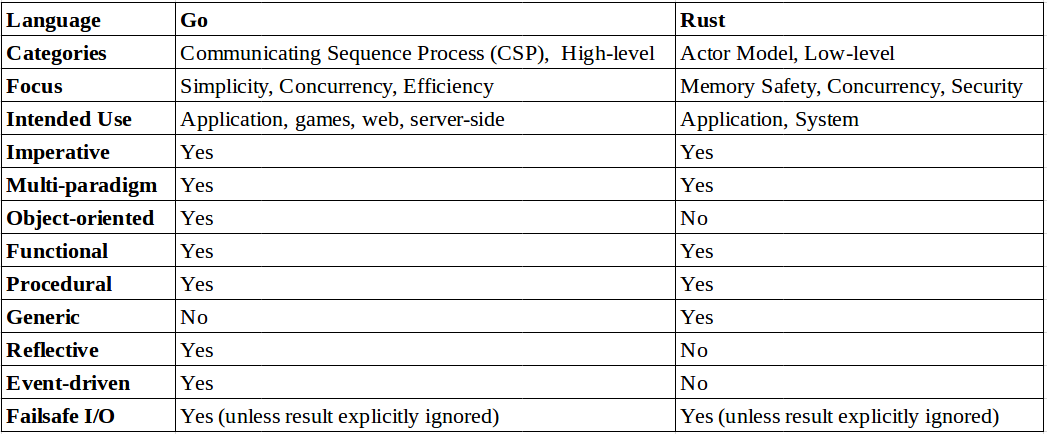
\includegraphics[width=1.0\textwidth]{Figure/go-vs-rust.png}
	\rule{35em}{0.5pt}
	\caption[Comparison of Go and Rust language characteristic]{Comparison of Go and Rust language characteristic}
\end{figure}

\subsection{Comparison of language categories and focus}

Go is a high-level language focus on simplicity, reliability and efficiency. The language is designed with communicating sequential process (CSP) to express concurrency based on message passing channels. The processes and messages communicate via goroutine and gochannel within a shared memory. \cite{go-csp} The language is intended to use for building web application programming interface (API) or networking application such as TCP or HTTP server to handle request.

Go possess simple syntax, garbage collector and runtime which allow developer to increase code readability and implement concurrency easier. However, Go is lack of language extensibility which leads to a limitation on implement manual memory management. \cite{go-problem}

\pagebreak

Rust is a low-level language focus on memory safety, security and fault tolerance. The language designed with actor model concurrent programming language that use “actors” as fundamental agent on message passing. The actor takes input, send output after performing functions. \cite{rust-actor-model} The processes and message communicate point-to-point via actors in a consistent state. The language intended use for system programmings such as building game engines, driver and embedded devices.

Rust doesn’t possess garbage collection and runtime which promote extensibility and deterministic on implement memory management. \cite{why-use-rust} However, Rust has much inherent complexity of syntax and semantics and has a high learning curve for a developer.
\pagebreak

\subsection{Similarities of Go and Rust language}

The similarities of both languages are discussed as follow: 

\begin{enumerate}[topsep=0pt,itemsep=-1ex,partopsep=1ex,parsep=1.5ex]
	
	\item \textbf{Imperative.} Go and Rust are imperative programming paradigm where a value can be assigned into a variable to perform operation on information located in memory. Moreover, these languages allow declaration of a variable to store the results in memory for later use, affect the global state of a variable.
	\item \textbf{Functional.} Go and Rust language can be written with mathematical functions to express control flow by combining function calls. The function avoid changing global state of variable. 
	\item \textbf{Procedural.} Go and Rust language can be written into statement structured and divided into function. The function known as procedure takes input processes it and produces output.
	\item \textbf{Multi-paradigm.} Go and Rust language are support various programming paradigm and provide developer to use suitable programming style to develop a program to achieve project objectives.
	\item \textbf{Failsafe I/O and callbacks.} Go and Rust language compiler warn error or throw an exception if the system calls fail. Go language throw errors if developer doesn’t use the declare function or variable and Rust language does not compile if found any dangling pointers.
	
\end{enumerate}
\pagebreak

\subsection{Difference between Go and Rust language}

The difference between both languages are discussed as follow: 

\begin{enumerate}[topsep=0pt,itemsep=-1ex,partopsep=1ex,parsep=1.5ex]
	
	\item \textbf{Object-oriented.} Go language support object-oriented programming with struct and interface. However, Rust is not an object-oriented language result of the idiomatic language and its appearance in an OO language. \cite{rust-not-oop}
	\item \textbf{Generic. } Go language is lack of generic where the compiler doesn’t allow declared a function or variable written in to-be-specified-later types await to be instantiated when needed for a specific purpose. However, Rust is possible to specify generalized function and avoid codes rewriting.
	\item \textbf{Reflective.} Go language possess the ability to observe and modify type, object, function execution on runtime by import “reflect”. However, Rust doesn’t have reflection.
	\item \textbf{Event-Driven. } Go is a high-level language enable write application respond to demand and expectation from mobile devices, multicore architectures and cloud computing environments. However,  Rust is a low-level language prevent the flow of program interrupt by an event from user actions to enforce security and safety. 
	
\end{enumerate}

\pagebreak

\section{Ubuntu 16.04.03 LTS 64-bit OS }

Ubuntu OS is an open source operating system with Linux distribution system and based on Debian architecture which provides long-term support (LTS) on security and fixes. \cite{difference-unix} The advantage of Ubuntu operating system are described below:

\begin{enumerate}[topsep=0pt,itemsep=-1ex,partopsep=1ex,parsep=1.5ex]
	
	\item \textbf{Free and customizable.} The openness of using Ubuntu OS offers a wide range of choices for the programmer to conduct development activities with Linux terminal. The APT packaging system allows developer to manage software and programming languages package efficient compared to Window operating system. The OS provides freedom in customization for a developer to catered different sets of need with source access and root permission to meet project requirements.
	\newline
	
	\item \textbf{Security.} The system files are owned by root in Ubuntu OS and not accessible by casual user, malware and third party software without root privilege. \cite{ubuntu-secure-than-window} As the operating system is maintained and contributed by vast amount of developer and programmer due to its open source and environment, the bugs are fixed efficiently with regular updates and provide less vulnerability for the attacker to exploit the system. \cite{linux-secure-than-window} The key factors underline within Ubuntu security provide sufficient statement to prove Ubuntu is more secure than Window or Mac OS on this project.	
	\newline
	
	\item \textbf{Consistent.} Ubuntu OS provide excellent consistent from front-end (UIUX) to back end. The user interface and user experience of Ubuntu operating system increase usability and efficiency in development, maintenance and deployment activities in the different version.
	\newline
	
	\item \textbf{Stable and Reliable.} UNIX preceded and outshine MS-DOS kernel with hardware abstraction, security model, resource management and various services that ran as background processes. \cite{difference-unix-msdos} Ubuntu promotes multitasking and multi-user which is suitable and ideal for this project to conduct concurrent and distributed processing activities with PostgreSQL. Last but not least, MS-DOS is an image loader system that preload memory addresses without memory or resource management quickly leads to BSOD and data corruption during data processing.
	
	
\end{enumerate}

\section{Debugging tools}

Debugging could be painful for a software engineer to monitor and identify the performance of applications running in concurrent and distributed on sophisticated operating systems like Ubuntu. 

Debugging with printf() for program bring many disadvantages and limitation during concurrency programming. The function could consume much memory in the multi-threaded environment because it’s not lightweight and thread safety. \cite{printf-bad} Moreover, it is not an efficient way to identify problems occurs related to memory allocation or interruption.

Therefore, debugger is used in this project to understand event or consequence happens in a running software system without consuming the enormous amount of memory. Simultaneously, it helps developer to save times on finding coding and logic errors in source codes.  \cite{what-is-tracing} 

\subsection{GDB Debugger}

GDB is a build in GNU debugger for UNIX systems to debug programs to obtain information of root cause that cause the program to fail. \cite{what-is-debugger} GDB allows set breakpoints and watchpoints on certain functions and print values during the program execution with terminal interface. Unfortunately, GDB possess limitation on finding bugs cause by memory leakage and compile errors.

\section{Eclipse for Parallel Application Developers Oxygen Release (4.7.0) IDE.} 

Eclipse is an integrated development environment create and maintain by Eclipse Open Source Project teams. The Eclipse Oxygen release possess better functionality and performance for a developer to manage, build and deploy software system. The advantage of Eclipse IDE are listed as follows: 

\begin{enumerate}[topsep=0pt,itemsep=-1ex,partopsep=1ex,parsep=1.5ex]
	
	\item \textbf{Auto Completion.} The openness of using Ubuntu OS offers a wide range of choices for the programmer to conduct development activities with Linux terminal. The APT packaging system allows developer to manage software and programming languages package efficient compared to Window operating system. The OS provides freedom in customisation for a developer to catered different sets of need with source access and root permission to meet project requirements.
	\newline
	
	\item \textbf{Integrated Environment. } The system files are owned by root in Ubuntu OS and not accessible by casual user, malware and third party software without root privilege. \cite{ubuntu-secure-than-window} As the operating system is maintained and contributed by vast amount of developer and programmer due to its open source and environment, the bugs are fixed efficiently with regular updates and provide less vulnerability for the attacker to exploit the system. \cite{linux-secure-than-window} The key factors underline within Ubuntu security provide sufficient statement to prove Ubuntu is more secure than Window or Mac OS on this project.	
	\newline
	
	\item \textbf{Debugger. } Ubuntu OS provide excellent consistent from front-end (UIUX) to backend. The user interface and user experience of Ubuntu operating system increase usability and efficiency in development, maintenance and deployment activities in the different version.
	\newline
	
	\item \textbf{Plugins.} UNIX preceded and outshine MS-DOS kernel with hardware abstraction, security model, resource management and various services that ran as background processes. \cite{difference-unix-msdos} Ubuntu promotes multitasking and multi-user which is suitable and ideal for this project to conduct concurrent and distributed processing activities with PostgreSQL. Last but not least, MS-DOS is an image loader system that preload memory addresses without memory or resource management quickly leads to BSOD and data corruption during data processing.
	
	
\end{enumerate}

\pagebreak

% MAIN SECTION ==============================
\section{Chapter Summary}

The finding for literature review is concurrent programming language possess specific built-in notation, package and functions to build parallel and distributed application. PostgreSQL is suitable for this project because it possesses MVCC that able handle concurrent request with good adaptivity and accuracy. Golang and Rust are concurrent programming language support multi-paradigm programming with multiprocessing and multithreading. Go language focused on simplicity while Rust language focuses on security. Both programming languages invented with different model and concepts for a different purpose.

Concurrent language is often compared and evaluated with configuration, categories and architecture to obtain performance and expressive power. The language's feature is essential to prove the performance of specific concurrent language. Debugging tools play a main role on observing processes and threads activities during the development and debugging activity to ensure program's execution is observed and error are discovered. 

